\chapter{Setup}
\label{app:setup}

\begin{figure}[htp]
  \centering
 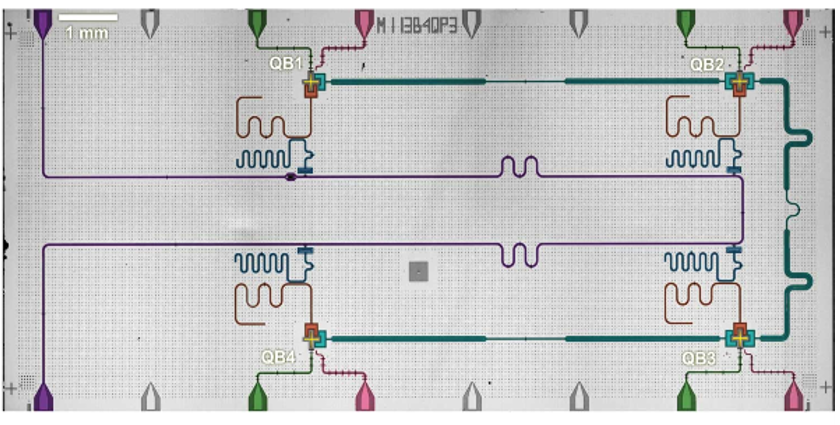
\includegraphics[width=0.8\textwidth]{appendices/figs/BF1_device.png}
 \caption{An optical micrograph of the 4-qubit device. Adapted from \cite{Andersen2019a}}
 \label{fig:BF1_device_picture}
\end{figure}

\begin{table}[ht]
\centering
\caption{Coherence, frequency, coupling, and readout properties of the device. The $T_1$ and $T_2$ times are measured at the maximum qubit frequency for qubit 1, and at the minimum qubit frequency for qubits 3 and 4. Qubit 2 is not tunable. Adapted from \cite{Andersen2019a}}
\begin{tabularx}{\textwidth}{llllll}
\toprule
Parameter & Unit & \textbf{Q1} & \textbf{Q2} & \textbf{Q3} & \textbf{Q4} \\ 
\midrule
Maximum qubit frequency & (GHz) & \multicolumn{1}{c}{5.721} & \multicolumn{1}{c}{5.210} & \multicolumn{1}{c}{5.530} & \multicolumn{1}{c}{5.160} \\
Minimum qubit frequency & (GHz) & 5.083 & 4.880 & 4.386 &  \\
Qubit lifetime & ($\mu$s) & 25.11 & 10.3 & 23.6 & 43.1 \\
Qubit Ramsey coherence time & ($\mu$s) & 23.87 & 11.3 & 14.2 & 10.7 \\
Qubit echo coherence time & ($\mu$s) & 34.8 & 12.1 & 19.5 & 20.2 \\
Readout resonator frequency & (GHz) & 6.892 & 7.087 & 6.687 & 6.487 \\
Purcell resonator – readout resonator detuning & (MHz) & 29.5 & 27.5 & 19.4 & 7.8 \\
Purcell resonator – readout resonator coupling & (MHz) & 10.9 & 8.2 & 9.5 & 10.4 \\
Purcell resonator to half-feedline coupling & (MHz) & 27.2 & 34.7 & 10.7 & 19.8 \\
Effective readout resonator linewidth & (MHz) & 2.4 & 2.0 & 1.5 & 6.1 \\
Dispersive shift & (MHz) & -3.9 & -1.6 & -1.8 & -2.4 \\
Thermal population & (\%) & 0.9 & 1.4 & 1.4 & 7.4 \\ 
\bottomrule
\end{tabularx}
\end{table}
